\documentclass{article}

\usepackage{graphicx}
\usepackage{float}

\usepackage{polski}
\usepackage[utf8]{inputenc}
\usepackage{indentfirst}

\usepackage{listings}

\usepackage{pdfpages}

% these 2 packages have to be used in this order
\usepackage{siunitx}
\usepackage{csvsimple}

\usepackage{mdframed}
\usepackage{alltt}

\usepackage{cite}
\usepackage{caption}

\usepackage{hyperref}

\usepackage{rotating}
\usepackage{tikz}

\AtBeginDocument{\renewcommand{\abstractname}{Abstrakt}}
\date{}
\renewcommand*{\figurename}{Rys.}
\renewcommand*{\tablename}{Tab.} 

\author{
Magdalena Jóźwiakowska\textsuperscript{1}\\\texttt{jozwiakowska@gmail.com}
\and
Mikołaj Buchwald\textsuperscript{1}\\\texttt{mikolaj.buchwald@gmail.com}
}
\title{Wykrywanie artefaktów mrugania w sygnale EEG przy pomocy Sztucznych Sieci Neuronalnych\\Dodatki}


\begin{document}

\maketitle
\textsuperscript{1} Grupa Robocza Inżynierii Kognitywistycznej \\
Instytut Psychologii Uniwersytetu im. Adama Mickiewicza w Poznaniu
\\

\begin{abstract}
    W niniejszej pracy podjęto kwestię użycia Sztucznych Sieci Neuronalnych (ang. Artificial Neural Network - ANN) w celu detekcji artefaktów mrugania w sygnale pochodzącym z elektroencefalografu (EEG). Dane przetwarzane na potrzeby projektu pochodzą z jedno-elektrodowego EEG MindWave Mobile firmy NeuroSky. Dane pobrano i podzielono na paczki za pomocą języka programowania Python. Do szkolenia ANN oraz kategoryzacji poszczególnych paczek sygnału wykorzystano bibliotekę języka programowania C - FANN (Fast Artificial Neural Network). Wykresy wygenerowano za pomocą programu Scilab.
\end{abstract}
% % % % %

%%%%%%%%%%%%%%%%%%%%%%%%%%%%%%%%%%%%%%%%%%%%%%%%%%%%%%%%%%%%%%%%
%    SUPPLEMENTS    SUPPLEMENTS    SUPPLEMENTS                 %
%%%%%%%%%%%%%%%%%%%%%%%%%%%%%%%%%%%%%%%%%%%%%%%%%%%%%%%%%%%%%%%%
    \newpage
    \section*{Dodatek A: Programy oraz skrypty}
        Wszystkie pliki potrzebne do przeprowadzenia eksperymentu oraz obróbki danych dostępne są w repozytorium Github: \\
            \url{https://github.com/mikbuch/eeg\_01\_mwm\_blink} \\

        \begin{enumerate}
            \item{Python, główna klasa służąca do podziału danych i ekstrakcji cech} \\
                \url{https://github.com/mikbuch/eeg\_01\_mwm\_blink/blob/master/EEGDataSplitMerge.py}

            \item{Python PsychoPy zbieranie danych do szkolenia ANN} \\
                \url{https://github.com/mikbuch/eeg\_01\_mwm\_blink/blob/master/psychopy\_experiment/psypy\_train.py}

            \item{Python podział danych i ekstrakcja cech dla etapu szkolenia} \\
                \url{https://github.com/mikbuch/eeg\_01\_mwm\_blink/blob/master/features\_train.py}

            \item{C FANN tworzenie oraz szkolenie Sztucznej Sieci Neuronalnej} \\
                \url{https://github.com/mikbuch/eeg\_01\_mwm\_blink/blob/master/fann\_eeg\_learn/eeg\_blink\_tra.c}

            \item{Python PsychoPy zbieranie danych do kategoryzacji przez ANN} \\
                \url{https://github.com/mikbuch/eeg\_01\_mwm\_blink/blob/master/psychopy\_experiment/psypy\_main.py}

            \item{Python podział danych i ekstrakcja cech dla etapu kategoryzacji} \\
                \url{https://github.com/mikbuch/eeg\_01\_mwm\_blink/blob/master/features\_categ.py}

            \item{C FANN kategoryzacja poszczególnych paczek danych} \\
                \url{https://github.com/mikbuch/eeg\_01\_mwm\_blink/blob/master/fann\_eeg\_learn/eeg\_blink\_cate.c}

            \item{Python generowanie danych do Scilab oraz wyników} \\
                \url{https://github.com/mikbuch/eeg\_01\_mwm\_blink/blob/master/plotting\_data/plot\_eeg\_blink\_categ.py}

            \item{Scilab generowanie wykresów i eksport do PDF} \\
                \url{https://github.com/mikbuch/eeg\_01\_mwm\_blink/blob/master/plotting\_data/scilab\_plot\_eeg\_01.sce}

            \item{Pomocnicze skrypty bash}
                \begin{itemize}
                    \item{C FANN kompilacja i uruchamianie programu szkolącego Sieć} \\
                        \url{https://github.com/mikbuch/eeg\_01\_mwm\_blink/blob/master/fann\_eeg\_learn/fann\_train.sh}
                    \item{C FANN kompilacja i uruchanianie programu do kategoryzacji} \\
                        \url{https://github.com/mikbuch/eeg\_01\_mwm\_blink/blob/master/fann\_eeg\_learn/fann\_categ.sh}
                    \item{Kontrola etapu szkolenia} \\
                        \url{https://github.com/mikbuch/eeg\_01\_mwm\_blink/blob/master/run\_train.sh}
                    \item{Kontrola etapu kategoryzacji} \\
                        \url{https://github.com/mikbuch/eeg\_01\_mwm\_blink/blob/master/run\_categ.sh}
                \end{itemize}
        \end{enumerate}

        Na Github znajduje się także pliki \LaTeX z wyświetlanym tutaj raportem:
            \url{https://github.com/mikbuch/eeg\_01\_mwm\_blink/blob/master/report\_eeg\_blk/prog\_lab\_mj\_mb\_project\_report.tex}
    % % %

    \newpage
    \section*{Dodatek B: Szczegółowe wyniki}
        Objaśnienia do tabeli dotyczących paczek oraz grupowania ich w mrugnięcia: 
        \begin{itemize}
            \item Nr paczki - numer paczki, która została skategoryzowana jako mrugnięcie.
            \item Względem bodźca - czy zasięg paczki pokrywa się z zasięgiem występowania bodźca czy nie. 
            \begin{itemize}
                \item[*] 0 - nie pokrywa się\
                \item[*] 1 - pokrywa się\
            \end{itemize}
            \item Numer mrugnięcia - grupowanie paczek w mrugnięcia na podstawie wcześniejszych założeń.
            \item Początek paczki - numer próbki, na której zaczyna się paczka skategoryzowana jako mrugnięcie.
            \item Koniec paczki - numer próbki, na której kończy się paczka skategoryzowana jako mrugnięcie. 
        \end{itemize}

        Zamieszczone zostały tutaj tabele z mrugnięciami już podzielonymi na paczki poprawnie oraz niepoprawnie skaregoryzowane. Pogrupowane też zostały owe paczki w poprawnie skategoryzowane mrugnięcia oraz niepoprawnie skategoryzowane mrugnięcia.

        \subsection*{Osoba pierwsza}
            \begin{table}[H]
                \captionsetup{justification=centering}
                \caption {Zbiory paczek poprawnie skategoryzowanych jako mrugnięcia. \\ Osoba 001}
                \begin{center}
                    \begin{tabular}{| p{1cm} | p{1.75cm} | p{1.75cm} | p{1.75cm} | p{1.75cm} |}
                        \hline
                        Nr paczki & Względem bodźca & Numer mrugnięcia & Początek paczki & Koniec paczki \\
                        \hline
                        \hline
                        01 & 1 & 1 & 1152 & 1278 \\ 
                        \hline
                        02 & 1 & 1 & 1280 & 1406 \\ 
                        \hline
                        03 & 0 & 1 & 1408 & 1534 \\ 
                        \hline
                        04 & 1 & 2 & 2816 & 2942 \\ 
                        \hline
                        05 & 0 & 2 & 2944 & 3070 \\ 
                        \hline
                        06 & 0 & 2 & 3072 & 3198 \\ 
                        \hline
                        07 & 1 & 3 & 4608 & 4734 \\ 
                        \hline
                        08 & 1 & 3 & 4864 & 4990 \\ 
                        \hline
                        09 & 0 & 3 & 4992 & 5118 \\ 
                        \hline
                        10 & 1 & 4 & 6400 & 6526 \\ 
                        \hline
                        11 & 1 & 5 & 10496 & 10622 \\ 
                        \hline
                        12 & 0 & 5 & 10624 & 10750 \\ 
                        \hline
                        13 & 1 & 6 & 12032 & 12158 \\ 
                        \hline
                        14 & 1 & 6 & 12160 & 12286 \\ 
                        \hline
                        15 & 1 & 7 & 15616 & 15742 \\ 
                        \hline
                        16 & 1 & 7 & 15744 & 15870 \\ 
                        \hline
                        17 & 1 & 8 & 17152 & 17278 \\ 
                        \hline
                        18 & 1 & 8 & 17280 & 17406 \\ 
                        \hline
                        19 & 1 & 9 & 18688 & 18814 \\ 
                        \hline
                        20 & 1 & 9 & 18816 & 18942 \\ 
                        \hline
                        21 & 1 & 10 & 20224 & 20350 \\ 
                        \hline
                        22 & 1 & 10 & 20352 & 20478 \\ 
                        \hline
                        23 & 1 & 11 & 21888 & 22014 \\ 
                        \hline
                        24 & 1 & 12 & 24448 & 24574 \\ 
                        \hline
                        25 & 0 & 12 & 24576 & 24702 \\ 
                        \hline
                        26 & 1 & 13 & 26496 & 26622 \\ 
                        \hline
                        27 & 0 & 13 & 26624 & 26750 \\ 
                        \hline
                        28 & 1 & 14 & 28032 & 28158 \\ 
                        \hline
                        29 & 0 & 14 & 28544 & 28670 \\ 
                        \hline
                    \end{tabular}
                \end{center}
            \end{table}

            \begin{table}[H]
                \captionsetup{justification=centering}
                \caption {Zbiory paczek niepoprawnie skategoryzowanych jako mrugnięcia. \\Osoba 001}
                \begin{center}
                    \begin{tabular}{| p{1cm} | p{1.75cm} | p{1.75cm} | p{1.75cm} | p{1.75cm} |}
                        \hline
                        Nr paczki & Względem bodźca & Numer mrugnięcia & Początek paczki & Koniec paczki \\
                        \hline
                        \hline
                        brak & brak & brak & brak & brak \\ 
                        \hline
                    \end{tabular}
                \end{center}
            \end{table}

            Zgodnie z wcześniej przyjętymi kryteriami dla osoby badanej 001 nie ma niepoprawnie skategoryzowanych mrugnięć.

        \newpage
        \subsection*{Osoba druga}
            \begin{table}[H]
                \captionsetup{justification=centering}
                \caption {Zbiory paczek poprawnie skategoryzowanych jako mrugnięcia. \\ Osoba 002}
                \begin{center}
                    \begin{tabular}{| p{1cm} | p{1.75cm} | p{1.75cm} | p{1.75cm} | p{1.75cm} |}
                        \hline
                        Nr paczki & Względem bodźca & Numer mrugnięcia & Początek paczki & Koniec paczki \\
                        \hline
                        \hline
                        01 & 1 & 1 & 1408 & 1534  \\
                        \hline
                        01 & 1 & 1 & 1408 & 1534  \\
                        \hline
                        02 & 1 & 1 & 1536 & 1662  \\
                        \hline
                        03 & 0 & 1 & 1664 & 1790  \\
                        \hline
                        04 & 1 & 2 & 2944 & 3070  \\
                        \hline
                        05 & 1 & 2 & 3072 & 3198  \\
                        \hline
                        06 & 1 & 2 & 3200 & 3326  \\
                        \hline
                        07 & 1 & 3 & 5120 & 5246  \\
                        \hline
                        08 & 1 & 3 & 5248 & 5374  \\
                        \hline
                        09 & 1 & 4 & 6656 & 6782  \\
                        \hline
                        10 & 1 & 4 & 6784 & 6910  \\
                        \hline
                        11 & 0 & 4 & 6912 & 7038  \\
                        \hline
                        12 & 1 & 5 & 9728 & 9854  \\
                        \hline
                        13 & 1 & 5 & 9856 & 9982  \\
                        \hline
                        14 & 1 & 6 & 11264 & 11390  \\
                        \hline
                        15 & 1 & 6 & 11392 & 11518  \\
                        \hline
                        16 & 0 & 6 & 11520 & 11646  \\
                        \hline
                        17 & 1 & 7 & 13824 & 13950  \\
                        \hline
                        18 & 1 & 7 & 13952 & 14078  \\
                        \hline
                        19 & 0 & 7 & 14080 & 14206  \\
                        \hline
                        20 & 1 & 8 & 16384 & 16510  \\
                        \hline
                        21 & 1 & 8 & 16512 & 16638  \\
                        \hline
                        22 & 0 & 8 & 16640 & 16766  \\
                        \hline
                        23 & 1 & 9 & 17920 & 18046  \\
                        \hline
                        24 & 1 & 9 & 18048 & 18174  \\
                        \hline
                        25 & 0 & 9 & 18176 & 18302  \\
                        \hline
                        26 & 1 & 10 & 22144 & 22270  \\
                        \hline
                        27 & 0 & 10 & 22272 & 22398  \\
                        \hline
                        28 & 1 & 11 & 23552 & 23678  \\
                        \hline
                        29 & 1 & 11 & 23680 & 23806  \\
                        \hline
                        30 & 0 & 11 & 23808 & 23934  \\
                        \hline
                        31 & 1 & 12 & 25216 & 25342  \\
                        \hline
                        32 & 1 & 13 & 26752 & 26878  \\
                        \hline
                        33 & 1 & 13 & 26880 & 27006  \\
                        \hline
                        34 & 0 & 13 & 27008 & 27134  \\
                        \hline
                        35 & 1 & 14 & 28288 & 28414  \\
                        \hline
                    \end{tabular}
                \end{center}
            \end{table}

            \begin{table}[H]
                \captionsetup{justification=centering}
                \caption {Zbiory paczek niepoprawnie skategoryzowanych jako mrugnięcia. \\Osoba 002}
                \begin{center}
                    \begin{tabular}{| p{1cm} | p{1.75cm} | p{1.75cm} | p{1.75cm} | p{1.75cm} |}
                        \hline
                        Nr paczki & Względem bodźca & Numer mrugnięcia & Początek paczki & Koniec paczki \\
                        \hline
                        \hline
                        01 & 0 & 1 & 128 & 254 \\
                        \hline
                        02 & 0 & 2 & 2688 & 2814 \\
                        \hline
                        03 & 0 & 3 & 6400 & 6526 \\
                        \hline
                        04 & 0 & 4 & 7168 & 7294 \\
                        \hline
                        05 & 0 & 5 & 8576 & 8702 \\
                        \hline
                        06 & 0 & 6 & 10240 & 10366 \\
                        \hline
                        07 & 0 & 7 & 13056 & 13182 \\
                        \hline
                        08 & 0 & 7 & 13312 & 13438 \\
                        \hline
                        09 & 0 & 8 & 13568 & 13694 \\
                        \hline
                        10 & 0 & 9 & 17024 & 17150 \\
                        \hline
                        11 & 0 & 10 & 24192 & 24318 \\
                        \hline
                        12 & 0 & 10 & 24320 & 24446 \\
                        \hline
                    \end{tabular}
                \end{center}
            \end{table}

        \subsection*{Osoba trzecia}
            \begin{table}[H]
                \captionsetup{justification=centering}
                \caption {Zbiory paczek poprawnie skategoryzowanych jako mrugnięcia. \\ Osoba 003}
                \begin{center}
                    \begin{tabular}{| p{1cm} | p{1.75cm} | p{1.75cm} | p{1.75cm} | p{1.75cm} |}
                        \hline
                        Nr paczki & Względem bodźca & Numer mrugnięcia & Początek paczki & Koniec paczki \\
                        \hline
                        \hline
                        01 & 1 & 1 & 1024 & 1150 \\
                        \hline
                        02 & 1 & 1 & 1152 & 1278 \\
                        \hline
                        03 & 0 & 1 & 1280 & 1406 \\
                        \hline
                        04 & 1 & 2 & 2560 & 2686 \\
                        \hline
                        05 & 1 & 2 & 2688 & 2814 \\
                        \hline
                        06 & 0 & 2 & 2816 & 2942 \\
                        \hline
                        07 & 1 & 3 & 4224 & 4350 \\
                        \hline
                        08 & 0 & 3 & 4352 & 4478 \\
                        \hline
                        09 & 1 & 4 & 6656 & 6782 \\
                        \hline
                        10 & 1 & 4 & 6784 & 6910 \\
                        \hline
                        11 & 0 & 4 & 6912 & 7038 \\
                        \hline
                        12 & 1 & 5 & 9344 & 9470 \\
                        \hline
                        13 & 0 & 5 & 9472 & 9598 \\
                        \hline
                        14 & 1 & 6 & 10880 & 11006 \\
                        \hline
                        15 & 1 & 7 & 12416 & 12542 \\
                        \hline
                        16 & 1 & 8 & 13952 & 14078 \\
                        \hline
                        17 & 1 & 8 & 14080 & 14206 \\
                        \hline
                        18 & 1 & 9 & 16000 & 16126 \\
                        \hline
                        19 & 1 & 9 & 16128 & 16254 \\
                        \hline
                        20 & 1 & 10 & 17536 & 17662 \\
                        \hline
                        21 & 1 & 10 & 17664 & 17790 \\
                        \hline
                        22 & 1 & 11 & 19584 & 19710 \\
                        \hline
                        23 & 1 & 11 & 19712 & 19838 \\
                        \hline
                        24 & 1 & 12 & 23168 & 23294 \\
                        \hline
                        25 & 1 & 12 & 23296 & 23422 \\
                        \hline
                        26 & 1 & 13 & 25728 & 25854 \\
                        \hline
                        27 & 1 & 13 & 25856 & 25982 \\
                        \hline
                        28 & 1 & 14 & 27264 & 27390 \\
                        \hline
                        29 & 1 & 14 & 27392 & 27518 \\
                        \hline
                    \end{tabular}
                \end{center}
            \end{table}

            \begin{table}[H]
                \captionsetup{justification=centering}
                \caption {Zbiory paczek niepoprawnie skategoryzowanych jako mrugnięcia. \\Osoba 003}
                \begin{center}
                    \begin{tabular}{| p{1cm} | p{1.75cm} | p{1.75cm} | p{1.75cm} | p{1.75cm} |}
                        \hline
                        Nr paczki & Względem bodźca & Numer mrugnięcia & Początek paczki & Koniec paczki \\
                        \hline
                        \hline
                        01 & 0 & 1 & 2048 & 2174 \\
                        \hline
                        02 & 0 & 2 & 4864 & 4990 \\
                        \hline
                        03 & 0 & 3 & 21376 & 21502 \\
                        \hline
                        04 & 0 & 4 & 27520 & 27646 \\
                        \hline
                    \end{tabular}
                \end{center}
            \end{table}

        \begin{sidewaysfigure}[p]
            \hspace*{-4.5cm} 
            \vspace*{1.5cm} 
            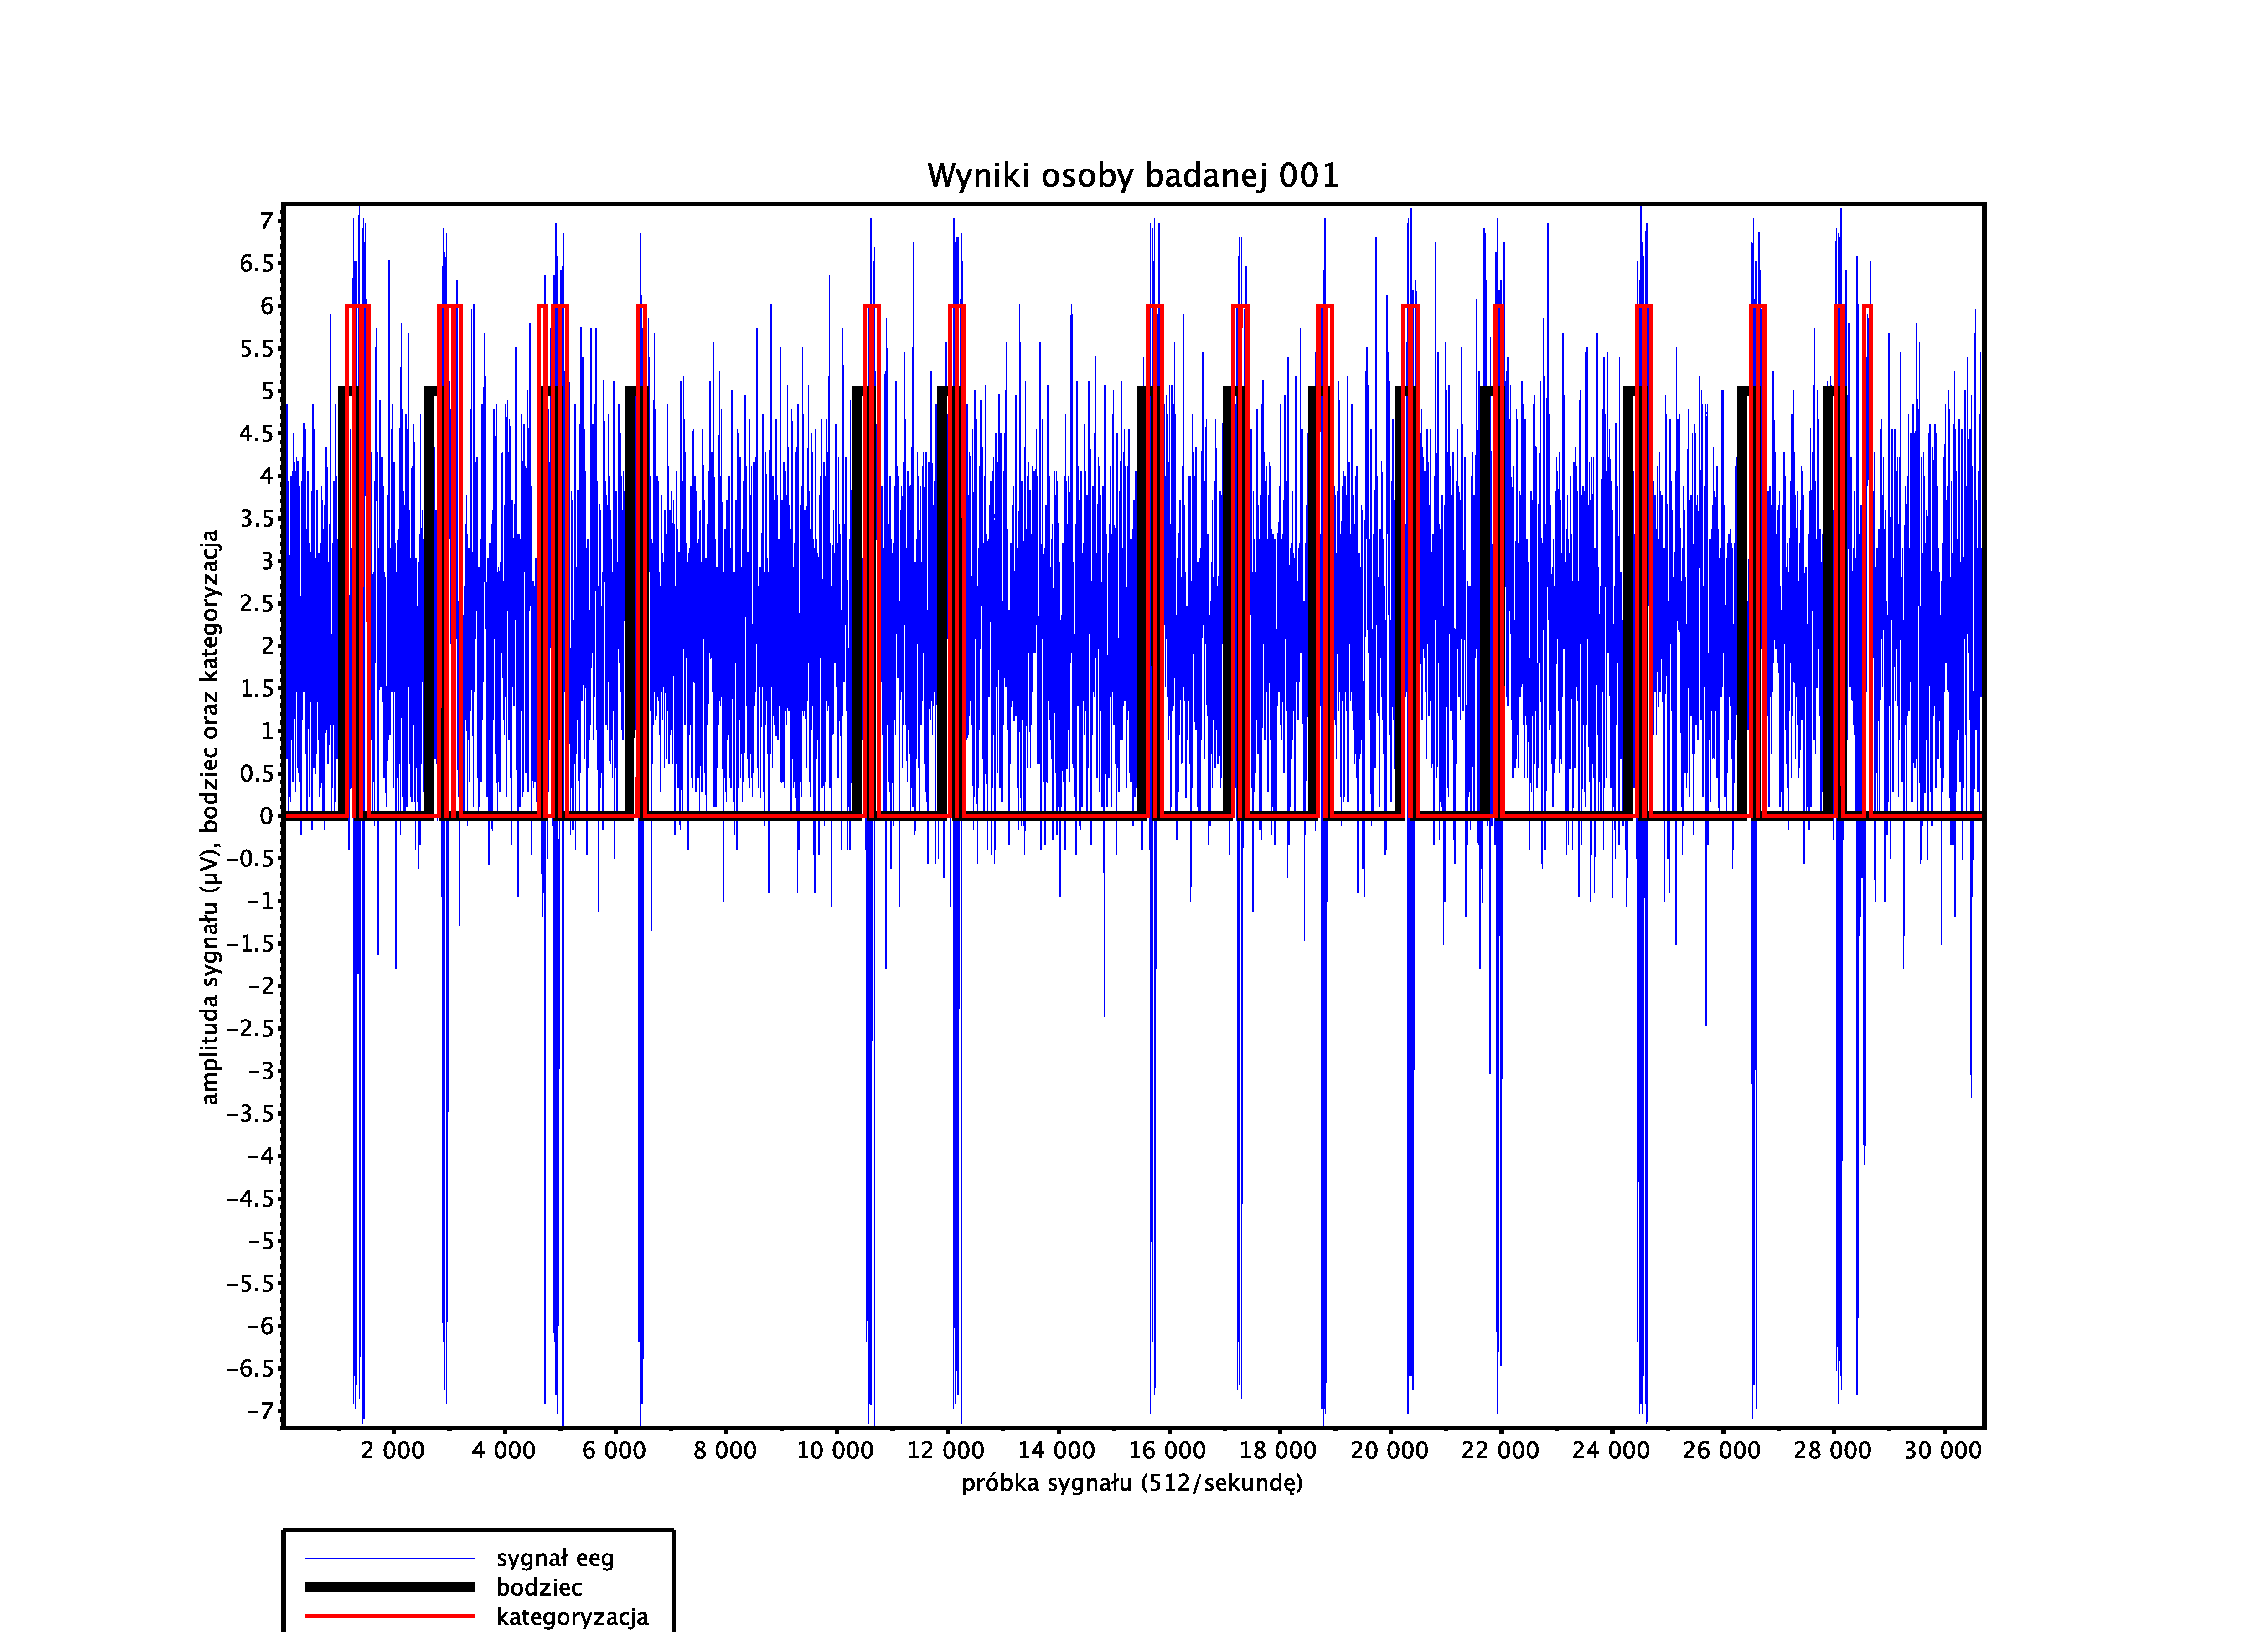
\includegraphics[width=\linewidth+10cm]{../plotting_data/scilab_eeg_01_sub_001.pdf}
            \caption{Dane dla osoby badanej 001}
        \end{sidewaysfigure}
        \begin{sidewaysfigure}[p]
            \hspace*{-4.5cm} 
            \vspace*{1.5cm} 
            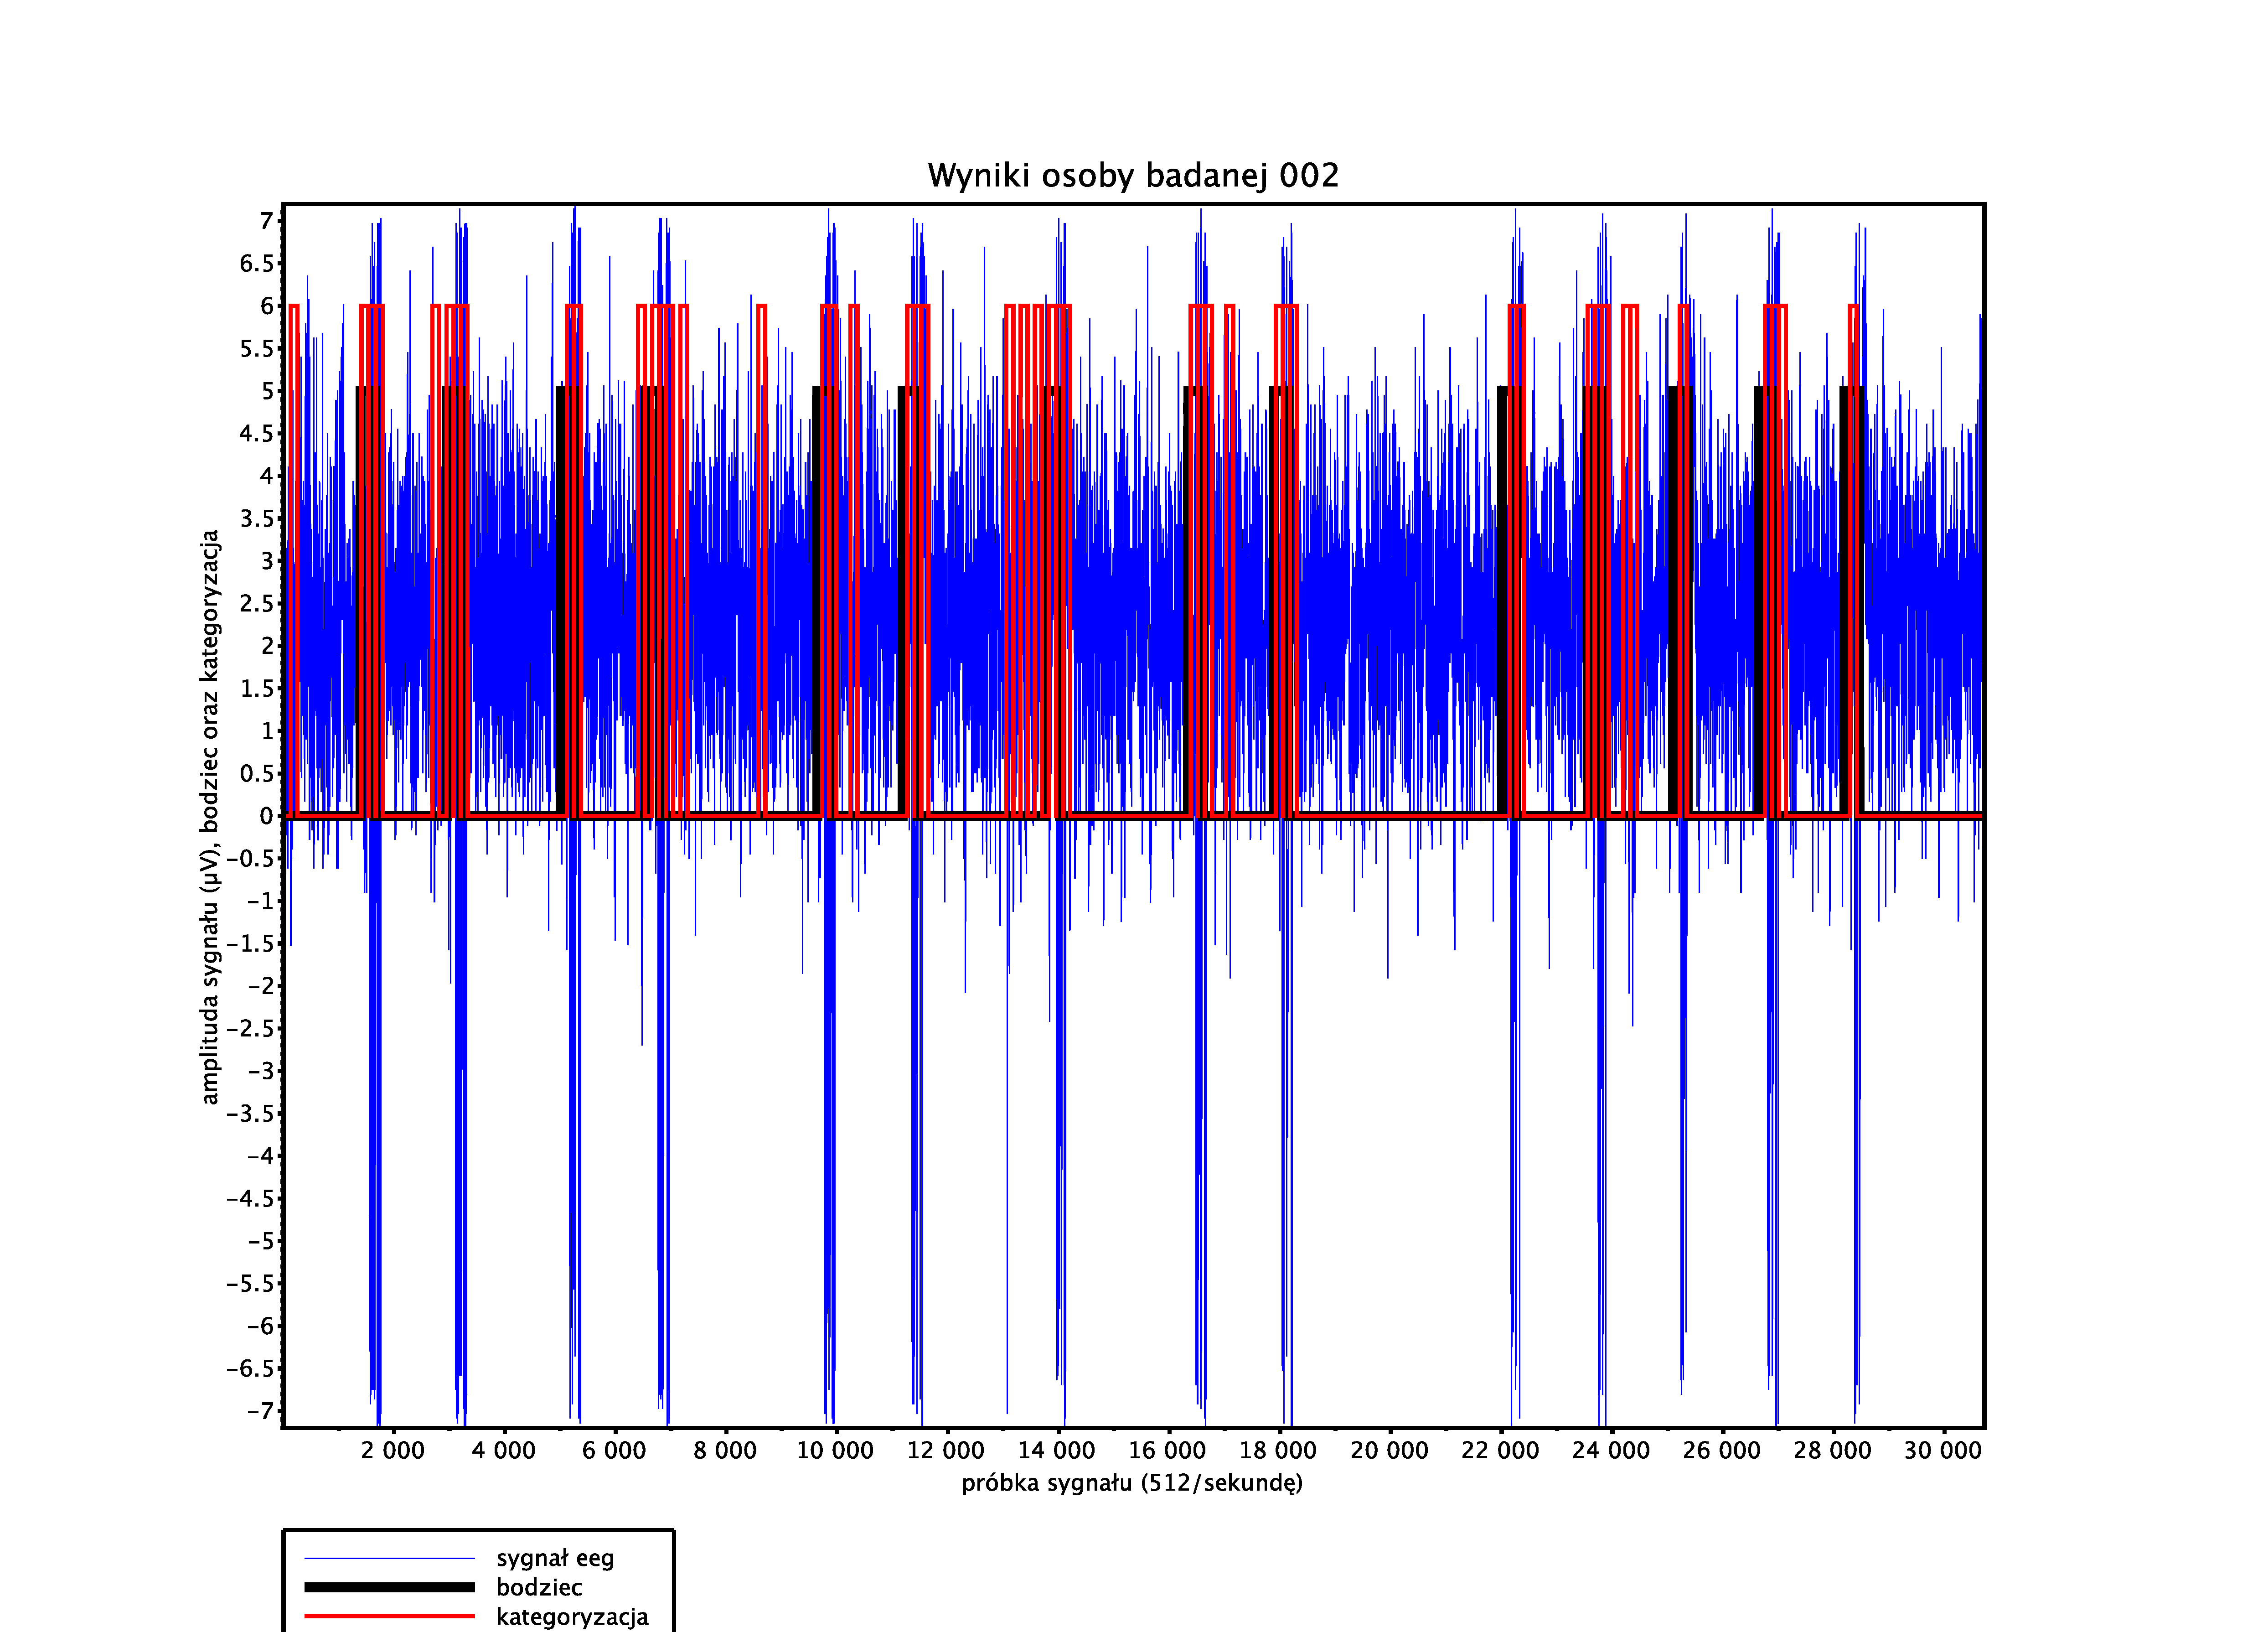
\includegraphics[width=\linewidth+10cm]{../plotting_data/scilab_eeg_01_sub_002.pdf}
            \caption{Dane dla osoby badanej 002}
        \end{sidewaysfigure}
        \begin{sidewaysfigure}[p]
            \hspace*{-4.5cm} 
            \vspace*{1.5cm} 
            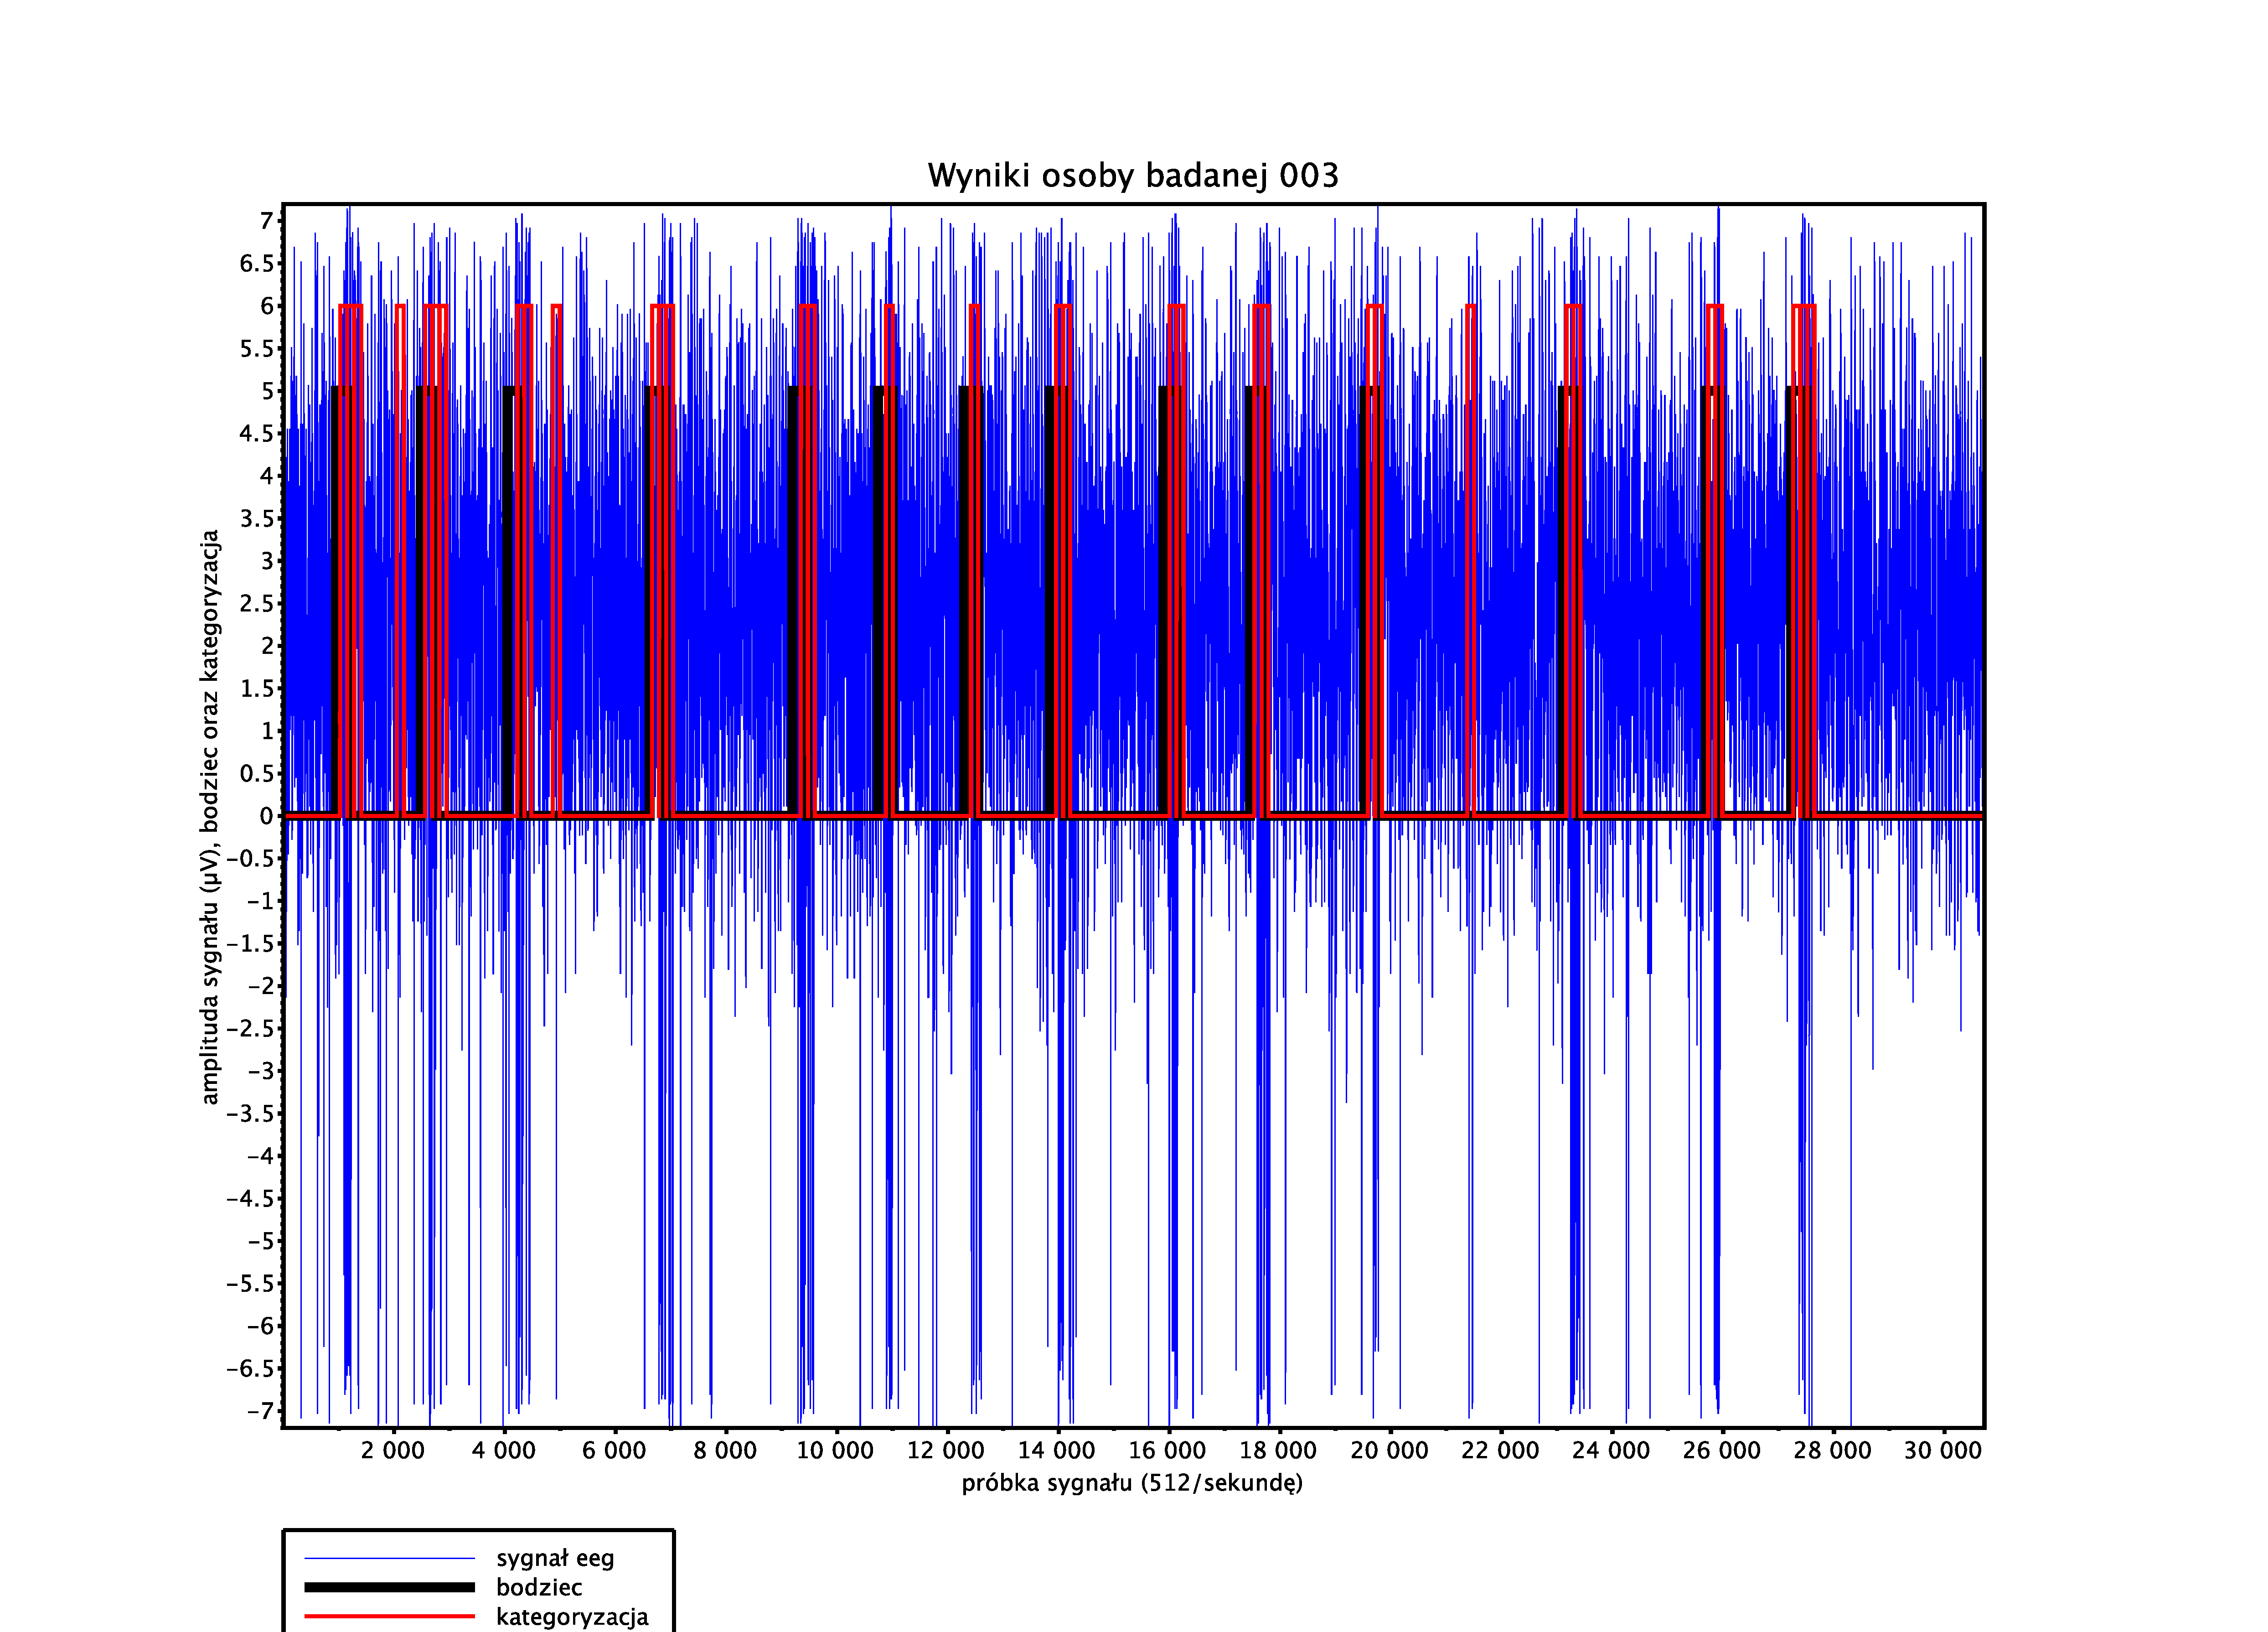
\includegraphics[width=\linewidth+10cm]{../plotting_data/scilab_eeg_01_sub_003.pdf}
            \caption{Dane dla osoby badanej 003}
        \end{sidewaysfigure}
    % % %

\end{document}
